\documentclass[11pt]{article}
\usepackage[a4paper,margin=1in]{geometry}
\usepackage[T1]{fontenc}
\usepackage{mathptmx}
\usepackage{microtype}
\usepackage{graphicx}
\setkeys{Gin}{keepaspectratio}
\usepackage{booktabs,longtable,array,calc}
\usepackage[font=small,labelfont=bf,labelsep=period]{caption}
\usepackage[hidelinks]{hyperref}
\usepackage{xurl}
\setlength{\parskip}{0.35em}
\setlength{\parindent}{0pt}
\providecommand{\tightlist}{\setlength{\itemsep}{0pt}\setlength{\parskip}{0pt}}
\def\LTcaptype{table}
\renewcommand{\arraystretch}{1.15}
\setlength{\LTpre}{0.6em}\setlength{\LTpost}{0.6em}
\title{\Large\textbf{Running AI models locally on a small budget: how software design made a cloned-voice lecture narrator practical on an ordinary CPU}}
\author{Xinhua Yu}
\date{November 2026}
\begin{document}
\maketitle
\begin{abstract}
\noindent \textit{Background.} Artificial intelligence models are now used mostly through
paid remote services, which charge for each use and receive the user's
data. Open-weight models are an alternative, but they are often assumed
to need a graphics processing unit (GPU). We tested this assumption by
narrating lecture videos in an instructor's cloned voice on a computer
without a GPU.

\textit{Methods.} We used Qwen3-TTS, an open-weight speech model, through
qwen3-tts.cpp, its C++ implementation, on a 15-watt, 6-core laptop
processor. We measured where the time went and revised the engine one
limiting resource at a time. Revisions that should not change the sound
had to reproduce the original waveform samples exactly; the others were
adopted only after listening. A 51-slide lecture of 578 sentences was
recorded with the revised engine and with Gemini TTS, a paid service.

\textit{Results.} The original engine needed 3.79 seconds of computation per
second of speech. The revised engine needed 1.25 for one sentence at a
time and 0.48 for 16 sentences processed together, about 8 times as
fast. Most of the gain came from arranging the work rather than from
faster arithmetic. With the final settings, the 51.7-minute lecture
video was recorded in 30.2 minutes (0.59 of its length) and finished in
31.4 minutes, at no cost per use. Gemini TTS needed 0.71 of the video's
length with one sentence per request and 0.29 with grouped requests, a
difference made by the application's design alone.

\textit{Conclusions.} A capable open-weight model did practical work on a
low-cost computer without the data leaving it. Most of the speed came
from software design and engineering rather than from hardware, and much
of that work remains open for other models and processors.

\end{abstract}
\begin{figure}[htbp]
\hypertarget{fig:visual}{%
\centering
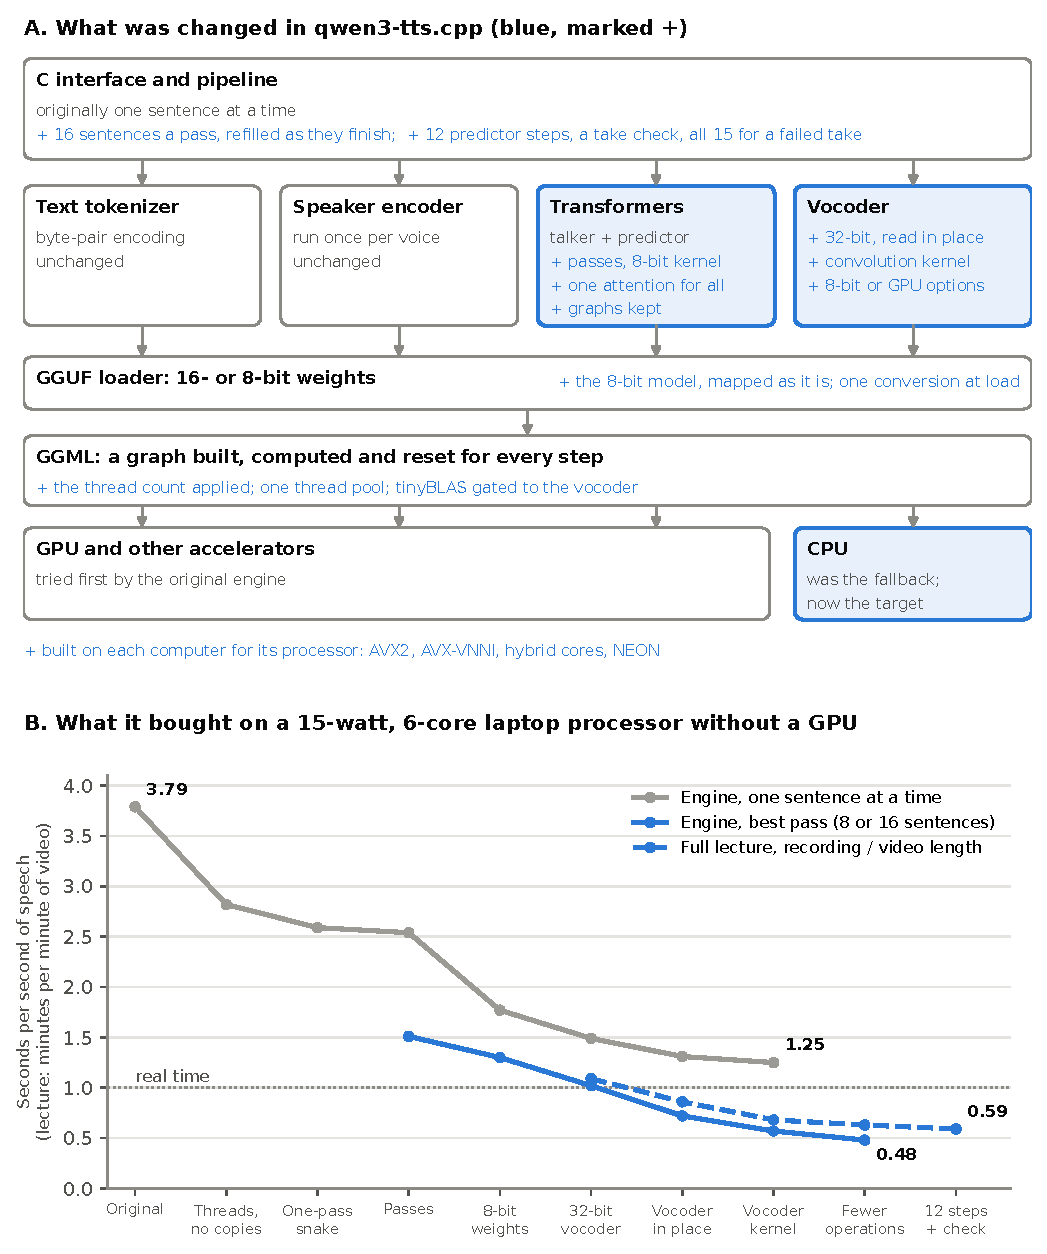
\includegraphics[width=1\textwidth,height=\textheight]{fig0_visual.pdf}
\caption{Visual abstract. (A) The parts of qwen3-tts.cpp and what was
changed in each; changes are in blue, marked +. (B) Speed as each group
of revisions was added: the engine one sentence at a time and in its
best pass (8 or 16 sentences), and the full 578-sentence lecture as
recording time over video length. Lower is faster; the dotted line marks
real time.}\label{fig:visual}
}
\end{figure}
\hypertarget{introduction}{%
\section{Introduction}\label{introduction}}

Artificial intelligence is now used in teaching and research mostly
through paid remote services. Language models draft and summarize text,
and speech models read it aloud, on servers that charge for each use.
This arrangement has costs beyond the fees. Data, including students'
work and instructors' voices, must leave the institution, and the work
depends on a provider's prices and terms. Open-weight models are an
alternative, but they are widely assumed to need a GPU and fast memory
that most instructors' computers lack.

Narrated lecture videos show the problem clearly. Revising a narrated
video is costly when every change must be recorded again. A cloned voice
removes this cost, since the instructor edits the text and the narration
is regenerated in the instructor's own voice. Hosted services can now
clone a voice from a short clip. Gemini TTS, for example, needs 10 to 30
seconds of speech and a spoken consent statement {[}4{]}. However, the
voice and every sentence of the lecture are then sent to the provider,
and each minute of audio is charged.

Qwen3-TTS, released by the Qwen team in January 2026 under the Apache
2.0 license, makes a local alternative possible {[}1{]}. It was trained
on more than 5 million hours of speech in 10 languages and clones a
voice from about 3 seconds of reference audio. Its smaller version, with
0.6 billion parameters, is small enough to run on a personal computer.
qwen3-tts.cpp reimplements this model in C++ on the GGML tensor library,
without Python or PyTorch at run time {[}2, 3{]}. Its author reported it
3.2 to 4.1 times as fast as the PyTorch version. On our test computer
without a GPU, however, it needed 3.79 seconds of computation for each
second of speech, so an hour of lecture took almost four hours.

Published work on the speed of speech synthesis has concentrated on GPU
servers, where the delay before the first audio and the number of
concurrent users are the main concerns. Less is known about what limits
such a model on a laptop processor, and how much of that limit is set by
the hardware rather than by the software. The question matters beyond
speech. Programs, including AI engines, are now often written quickly
and judged by whether they work, not by how well they use the computer.
If a large share of the time is lost in the software, much of the case
for remote services and new hardware rests on a gap that engineering
could close.

In this study, we examined whether a cloned-voice narrator can run on an
ordinary computer at a practical speed, and how much of the required
speed comes from software design. We identified the properties of the
model and its implementation that limit speed without a GPU. We then
revised the implementation one limiting resource at a time, keeping its
output identical wherever a change should not alter the sound. Finally,
we recorded a full lecture with the revised engine and with Gemini TTS.
Our aim is less to present a faster engine than to show what careful
design and measurement can achieve. We also draw lessons for running
other models, including language models, on limited hardware. The
revised engine is published as realme-qwen3-tts.cpp {[}7{]}, and every
revision can be switched off for comparison.

\hypertarget{the-model-and-the-engine}{%
\section{The model and the engine}\label{the-model-and-the-engine}}

\hypertarget{qwen3-tts}{%
\subsection{Qwen3-TTS}\label{qwen3-tts}}

Qwen3-TTS treats speech synthesis as language modeling, in which speech
is predicted as a sequence of discrete audio tokens (Figure 2). Since
the word ``code'' has several senses in this field, we name the unit at
each step. A text token is a unit of text from the Qwen tokenizer. An
audio frame is 80 ms of speech, so one second holds 12.5 frames. An
audio token is one value in a frame, an index into a codebook of 2,048
entries. Each frame holds 16 audio tokens: one semantic token, which
carries mainly what is said, and 15 acoustic tokens, which add the
detail of the voice in successive layers. Waveform samples are the audio
itself, 24,000 a second. In this paper, ``code'' refers only to program
code.

\begin{figure}[tbp]
\hypertarget{fig:model}{%
\centering
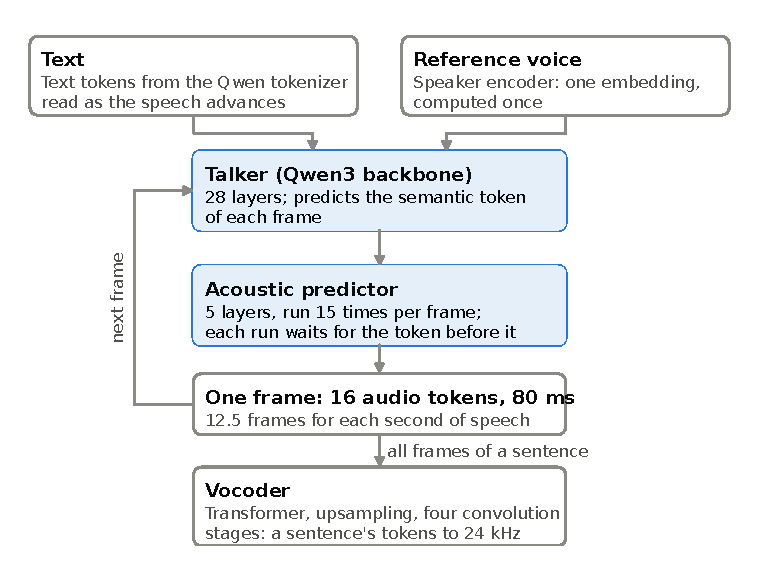
\includegraphics[width=0.85\textwidth,height=\textheight]{fig1_model.pdf}
\caption{The Qwen3-TTS 12 Hz model. Each frame takes one talker step for
the semantic token and 15 dependent runs of the acoustic predictor; the
vocoder turns a sentence's audio tokens into waveform
samples.}\label{fig:model}
}
\end{figure}

Two transformers predict the audio tokens, and a third network turns
them into sound. The talker, the Qwen3 language-model backbone with 28
layers, predicts each frame's semantic token from the text and the
previous frame. The acoustic predictor, with 5 layers of the same width,
then predicts the 15 acoustic tokens one after another, each run
conditioned on the token before. The vocoder looks up each audio token
in its codebook. A small transformer and four convolutional stages then
raise the rate from 12.5 to 24,000 values a second. The voice enters
once, as a speaker embedding computed from the instructor's reference
recording.

\hypertarget{the-qwen3-tts.cpp-engine}{%
\subsection{The qwen3-tts.cpp engine}\label{the-qwen3-tts.cpp-engine}}

qwen3-tts.cpp reproduces the Python pipeline as separate libraries over
one tensor library (Figure 1A). A text tokenizer, a speaker encoder, the
two transformers and the vocoder are each a library, and a C interface
joins them. A shared loader reads the weights from GGUF files in 16 or 8
bits. Every step builds a GGML computation graph, computes it and resets
it, so one frame involves 16 graphs. The engine prefers any GPU and uses
the CPU only as a fallback. We kept this structure: every revision sits
inside an existing part, and the original engine can still be built for
comparison. Figure 1B shows what the revisions bought, step by step.

\hypertarget{why-speed-depends-on-hardware}{%
\subsection{Why speed depends on
hardware}\label{why-speed-depends-on-hardware}}

Several properties of the model and its implementations make its speed
depend on hardware that most instructors do not have. Each became a
target of revision.

First, audio-token generation needs fast memory more than fast
arithmetic. With 8-bit weights, each frame reads about 1.76 GB of
weights and performs about two multiply-adds per byte read. About 73\%
of both falls in the acoustic predictor, because its 5 layers run 15
times a frame. Real-time speech for one sentence therefore needs about
22 GB of memory reads per second, close to what dual-channel DDR4 memory
sustains. A GPU reads its memory at several hundred gigabytes a second.

Second, the audio tokens of a frame are predicted strictly in sequence.
Each of the 15 runs of the acoustic predictor waits for the token
before, and the next frame waits for all 16. Each run is a small
matrix-vector product followed by synchronization of the threads, which
a GPU hides with fast scheduling and a CPU pays for at every step.

Third, the vocoder is heavy in arithmetic. Its convolutions need about
61 billion floating-point operations per second of speech. It reuses
small weights many times, so it is limited by arithmetic rather than by
memory, the opposite of generation.

Fourth, the implementation was designed for one streaming request on a
GPU. The original engine preferred any GPU and used the CPU as a
fallback, and it synthesized one sentence at a time. For narration,
where every sentence is known in advance, throughput matters and the
delay before the first audio hardly at all.

We used the 0.6-billion-parameter model rather than the 1.7-billion one.
In the technical report's multilingual test, its English error rate and
speaker similarity were no worse than the larger model's (word error
rate 0.84\% vs 0.93\%; similarity 0.83 vs 0.78) {[}1{]}. Its
transformers, however, read about a third as many bytes per frame. For
CPU-only English narration, the smaller model was the practical choice.

\hypertarget{methods}{%
\section{Methods}\label{methods}}

\hypertarget{test-computer-and-measures}{%
\subsection{Test computer and
measures}\label{test-computer-and-measures}}

All measurements were made on an Intel NUC with an i7-10710U processor
(15 W, 6 cores and 12 threads), 64 GB of DDR4-2667 memory and no
discrete GPU. The engine was built for AVX2 with Microsoft's compiler on
Windows. The application was RealMe Studio, which turns a slide deck and
its narration into a captioned video in the instructor's voice.

We used four measures. Speed was measured as the real-time factor,
seconds of computation per second of speech, so that values below 1.0
are faster than real time. For Gemini TTS, the corresponding quantity is
seconds of waiting per second of speech. For a whole lecture, we report
the recording time as a share of the video's length, which includes
pauses between sentences and slides. The effect of a revision on the
sound was measured with random sampling switched off. It is the
difference between the revised and original waveform samples, in
decibels below the level of the speech. For lossy options, we also
computed PESQ, a standard objective score of speech quality on a scale
up to 4.5, against the full-precision take {[}5{]}. Finally, we listened
to the same sentences recorded each way.

\hypertarget{the-recording-pipeline}{%
\subsection{The recording pipeline}\label{the-recording-pipeline}}

Recording a lecture involves five stages: preparing the text, computing
the speaker embedding, generating the audio tokens, decoding them to
waveform samples, and assembling the video (Figure 3). Only generation
and decoding are heavy. The other three stages, however, decide how much
of that work has to be done at all.

\begin{figure}[tbp]
\hypertarget{fig:pipeline}{%
\centering
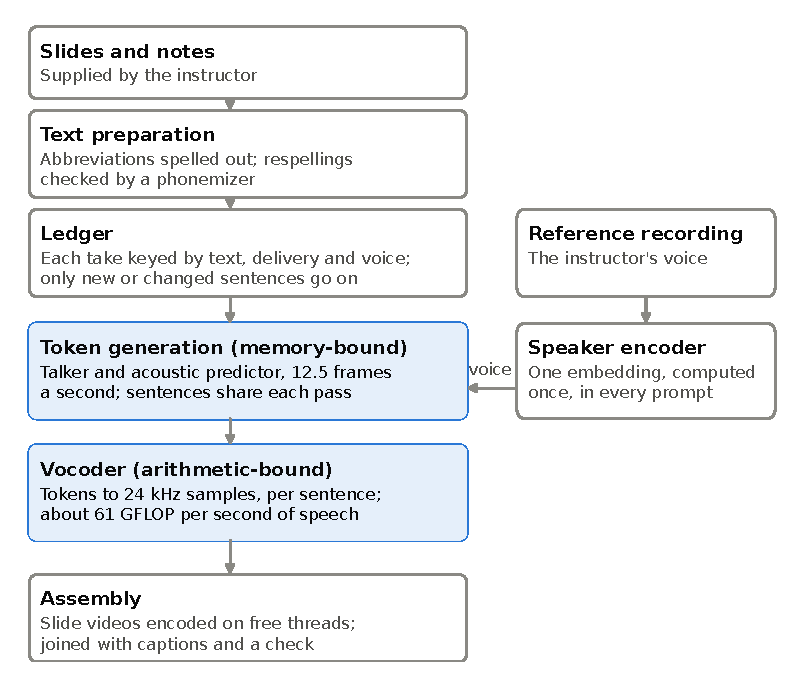
\includegraphics[width=0.8\textwidth,height=\textheight]{fig2_pipeline.pdf}
\caption{The recording pipeline. The voice enters once, as a speaker
embedding; the ledger passes only new or changed sentences to the two
heavy stages, which are limited by different
resources.}\label{fig:pipeline}
}
\end{figure}

Text is prepared as it will be spoken before any audio is produced.
Abbreviations are spelled out letter by letter unless they are on a
short list of terms people say as words, and a lexicon of respellings,
checked by a phonemizer, overrides both rules. The speaker embedding is
computed once and inserted into every sentence's prompt, so a voice
costs one vector and no time per sentence. Each recorded sentence, a
take, is entered in a ledger keyed by its text, its delivery and a
fingerprint of the voice, settings and model. An edited lecture
therefore re-records only the sentences that changed. The remaining
sentences go to the engine in passes, groups of sentences processed
together at each step. Each slide's video is encoded as soon as its
audio is complete, on the threads the engine leaves free.

\hypertarget{how-the-engine-was-revised}{%
\subsection{How the engine was
revised}\label{how-the-engine-was-revised}}

We followed four rules, chosen because each makes the next revision
cheaper to test. First, measure before changing anything, stage by
stage, since a whole-pipeline time hides which resource sets the pace.
Second, address one limiting resource at a time, because generation and
the vocoder were limited by different resources and needed different
remedies. Third, require exact output wherever a change should not alter
the sound. Such a revision had to reproduce the original waveform
samples with sampling off, and a sentence in a pass had to equal the
same sentence alone. Fourth, give every revision a run-time switch, so
that it can be turned off and compared on the same sentences.

Revisions were tested at three levels. Native tests compared each new
routine with GGML's own arithmetic on synthetic models with the real
shapes. Short timing tests on the NUC ran 16 sentences under each
setting, repeated in shuffled and reversed order, and required identical
audio from every run. The most promising settings were then confirmed on
a full lecture. Revisions that change the sound by design, such as fewer
acoustic tokens or 8-bit vocoder arithmetic, were adopted only after
listening tests on the NUC.

The engine was developed with AI coding assistants. Most of the program
investigation, coding and testing was done by Claude Code, with a second
assistant (Codex) carrying out several experiments and an independent
model reviewing the code. The measurements decided what was kept.

\hypertarget{revisions-of-the-engine}{%
\section{Revisions of the engine}\label{revisions-of-the-engine}}

The revisions kept fall into five groups: arranging the work, removing
waste, a convolution kernel for the vocoder, fewer and larger
operations, and stages tuned by listening (Table 1). Table 2 lists what
was tried and not kept.

\hypertarget{arranging-the-work}{%
\subsection{Arranging the work}\label{arranging-the-work}}

The largest gain came from letting several sentences share each read of
the weights. Since one sentence is limited by the bytes it reads, a pass
reads each weight once per step and applies it to every sentence in the
pass. Each sentence keeps its own attention cache, sampling and stopping
point, so its waveform samples are identical to those it would have
alone. With 16-bit weights, passes of eight sentences reduced the
real-time factor from 2.54 to 1.51.

A pass of fixed membership wastes capacity, because it lasts as long as
its longest sentence. On a real script, passes filled in slide order
lost about 20\% of generation time to empty places. We therefore refill
a place as soon as its sentence ends, so that the next sentence starts
at the following step. We call such a pass a stream. Streams were 9\%
faster than fixed passes on mixed sentences.

8-bit weights halve the bytes read per step. One sentence at a time went
from 2.54 to 1.77 seconds per second of speech, and passes of four from
1.66 to 1.35. 8-bit weights make a different model rather than a rounded
version of the same one, but in side-by-side listening the two were not
told apart. Within a pass, GGML loaded each 8-bit weight row again for
every sentence. We wrote a kernel that loads each row once for all
sentences, with exactly GGML's arithmetic, and it saved 16\% of the time
of a pass of eight on a 2-core computer.

\hypertarget{removing-waste}{%
\subsection{Removing waste}\label{removing-waste}}

Several revisions removed work that the original engine did for no
benefit. The requested thread count was stored but never passed to GGML,
so every computation ran on 4 threads whatever the computer; applying it
gave 1.26 times the speed on 6 cores. One weight matrix in each layer
was converted from 16 to 32 bits inside every step, about 1,240
conversions per second of speech, and is now converted once at load. The
vocoder copied per-channel values out to the length of the signal before
multiplying by them, and computed its activation function in five passes
over the signal. Removing these took the engine from 3.79 to 2.59
seconds per second of speech one sentence at a time. With the C
library's sine, none of them changed a sample; the faster sine used by
default moved the output about 70 dB below the speech.

The vocoder's own arithmetic was then rearranged. It had rounded its
signal to 16 bits at every layer and unrolled each convolution's input
sevenfold into a copy. We moved it to 32 bits and expressed its
transposed convolutions as single matrix products. We also laid the
signal out so that a 7-tap convolution reads its inputs in place rather
than from a copy. These steps reduced the vocoder's time from 0.80 to
0.26 seconds per second of speech and its working memory by two thirds.
Its output moved 50 to 60 dB below the speech, about what reordering a
32-bit sum produces through thirty layers.

\hypertarget{a-convolution-kernel-for-the-vocoder}{%
\subsection{A convolution kernel for the
vocoder}\label{a-convolution-kernel-for-the-vocoder}}

Once generation was shared across sentences, the vocoder took about half
the time, since it shares nothing between sentences. We wrote a
convolution kernel for it. The kernel reads each tap's rows in place and
multiplies them in tiles held in registers. It applies the bias,
residual addition and next activation as rows leave it, so a whole
residual unit is one operation. It reduced the vocoder's time from 0.26
to 0.19 seconds per second of speech, at about 80\% of the processor's
peak arithmetic on a 2-core test computer. Its innermost tile, like that
of the 8-bit pass kernel, is processor-specific: it exists in AVX2 for
x86 and NEON for 64-bit ARM, each with a portable version beside it.
Without these processor-specific tiles, the engine kept about 80\% of
its speed in passes of eight (0.74 vs 0.58).

\hypertarget{fewer-and-larger-operations}{%
\subsection{Fewer and larger
operations}\label{fewer-and-larger-operations}}

Timing each stage showed that, after the earlier revisions, the acoustic
predictor spent its time on many small operations rather than on
arithmetic. In a stream of 16 sentences, its 15 graphs held about 19,940
operations per frame, almost all of them one attention operation per
sentence per layer. Building these graphs took 5.9\% of the time. The
sentences in a pass all stand at the same step of the same frame, and
the predictor's attention spans one frame only. One attention operation
per layer can therefore serve every sentence, applied slice by slice
with GGML's own operations, so the numbers are unchanged. This cut the
predictor's operations per step from 19,940 to 3,440. Since a predictor
graph now depends only on the number of sentences and the pass's cache,
its 15 graphs are built once and reused frame after frame. A second
change gathers the talker's attention inputs in order before the
product. Later, the talker's graph was also kept from step to step,
checked by native tests; building it had taken 2\% to 3\% of the time.

The predictor changes and the ordered talker attention were exact: in 38
timed runs on the NUC, every run gave identical audio. Together they
reduced the time of a 16-sentence stream by 15\% (Section 5.2). None of
them made any arithmetic faster. They removed the cost of organizing the
arithmetic, which a GPU absorbs and a laptop processor pays at every
step.

\hypertarget{stages-tuned-by-listening}{%
\subsection{Stages tuned by listening}\label{stages-tuned-by-listening}}

Every stage of the model can be tuned, and some tunings change the sound
in ways only listening can judge. The acoustic predictor's 15 runs fill
codebooks from coarse to fine. We tested stopping after 12, 10 or 8 runs
and filling the rest with each codebook's mean value. In listening on
the NUC, 12 runs could not be told from 15, 10 were acceptable, and 8
were consistently worse. With zero fill instead of the mean, one
sentence at 8 runs ran on past its text, to 3.75 times its length.
Twelve runs reduced the predictor's time in one test from 6.4 to 5.1
seconds. Since the predictor takes about a third of the total, the
saving on a lecture should be a few percent.

We made 12 runs the default for passes and streams and kept 15 as a
fallback; a sentence recorded on its own always uses 15. The fallback is
triggered by a take check, which examines every take recorded in a pass
or stream before it is kept. It flags a take that ran on past its text
or holds invalid samples. It also flags a take far shorter than its
words need, mostly silent, stopping for more than 2 seconds, or clipped.
The check works on samples already in memory and takes about a
millisecond. A flagged take is recorded again on its own with all 15
runs. On the 78 takes of two listening tests, it flagged only the one
that ran on.

Two vocoder options were measured and kept off by default. Rounding the
vocoder's convolutions to 8 bits gave a PESQ of 4.48 against the 32-bit
vocoder but was no faster on the NUC's AVX2 processor. With 7-bit inputs
the vocoder was about 1.2 times as fast (5.2 vs 6.4 s in one run) at a
PESQ of 4.23. On processors with integer dot-product instructions
(AVX-VNNI), the 8-bit form was about 1.6 times as fast in a synthetic
test, so it is a candidate default for newer computers. The vocoder can
also run on a GPU through Vulkan, while the transformers stay on the
CPU; this was checked only on a software GPU.

\hypertarget{building-and-maintaining-one-engine}{%
\subsection{Building and maintaining one
engine}\label{building-and-maintaining-one-engine}}

The engine is built on each user's computer, for that computer's
processor, by the application itself. The build detects AVX-VNNI and
compiles bit-identical kernels that use it, and it shares the rows of
each 8-bit product between fast and slow cores on hybrid processors,
after a self-check. Neither applies to the NUC, whose processor has
neither feature, but both switch on by themselves on newer Intel
processors.

During development, the work had produced three builds of the revised
engine: one built the older way, a new build reading the standard model
files, and a version that read a separately prepared model bundle. A
matched test found no difference in speed between them (ratios to the
older build 1.016 and 1.017, 3 rounds, identical audio). We therefore
kept one engine, which reads the standard 8-bit model files directly,
and removed the bundle, its packed weight layouts and their tests. This
took about 1,100 lines (18\%) out of RealMe's own engine code without
changing a single audio token. The removal was checked by comparing the
audio tokens of the same synthetic sentences before and after, with
every native test passing.

\begin{longtable}[]{@{}
  >{\raggedright\arraybackslash}p{(\columnwidth - 6\tabcolsep) * \real{0.1707}}
  >{\raggedright\arraybackslash}p{(\columnwidth - 6\tabcolsep) * \real{0.3415}}
  >{\raggedright\arraybackslash}p{(\columnwidth - 6\tabcolsep) * \real{0.2683}}
  >{\raggedright\arraybackslash}p{(\columnwidth - 6\tabcolsep) * \real{0.2195}}@{}}
\caption{Revisions kept, the limit each addresses, and their effect on
the samples.}\tabularnewline
\toprule\noalign{}
\begin{minipage}[b]{\linewidth}\raggedright
Group
\end{minipage} & \begin{minipage}[b]{\linewidth}\raggedright
Revision
\end{minipage} & \begin{minipage}[b]{\linewidth}\raggedright
Limit addressed
\end{minipage} & \begin{minipage}[b]{\linewidth}\raggedright
Effect on samples
\end{minipage} \\
\midrule\noalign{}
\endfirsthead
\toprule\noalign{}
\begin{minipage}[b]{\linewidth}\raggedright
Group
\end{minipage} & \begin{minipage}[b]{\linewidth}\raggedright
Revision
\end{minipage} & \begin{minipage}[b]{\linewidth}\raggedright
Limit addressed
\end{minipage} & \begin{minipage}[b]{\linewidth}\raggedright
Effect on samples
\end{minipage} \\
\midrule\noalign{}
\endhead
\bottomrule\noalign{}
\endlastfoot
Arranging the work & several sentences per pass, refilled as they end &
weights read once per sentence; empty places & identical \\
Arranging the work & 8-bit weights; one weight-row load for the whole
pass & bytes read per step & different model, not told apart; kernel
identical \\
Removing waste & thread count applied; one conversion at load; no copies
& defects and repeated work & identical \\
Removing waste & 32-bit vocoder read in place & 16-bit rounding;
sevenfold copies & 50 to 60 dB below the speech \\
Vocoder kernel & fused tiles in registers & general-purpose products &
about 110 dB from previous \\
Fewer operations & one predictor attention for all sentences; kept
graphs; ordered talker attention & thousands of small operations per
step & identical \\
Tuned by listening & 12 predictor runs, 15 as fallback after a take
check & predictor runs per frame & not told apart in listening \\
Build & per-computer build; VNNI and hybrid-core kernels & processor
features & identical \\
\end{longtable}

\begin{longtable}[]{@{}
  >{\raggedright\arraybackslash}p{(\columnwidth - 4\tabcolsep) * \real{0.2639}}
  >{\raggedright\arraybackslash}p{(\columnwidth - 4\tabcolsep) * \real{0.3889}}
  >{\raggedright\arraybackslash}p{(\columnwidth - 4\tabcolsep) * \real{0.3472}}@{}}
\caption{Ideas tried and not kept, and why.}\tabularnewline
\toprule\noalign{}
\begin{minipage}[b]{\linewidth}\raggedright
Idea
\end{minipage} & \begin{minipage}[b]{\linewidth}\raggedright
What was measured
\end{minipage} & \begin{minipage}[b]{\linewidth}\raggedright
Why it did not pay
\end{minipage} \\
\midrule\noalign{}
\endfirsthead
\toprule\noalign{}
\begin{minipage}[b]{\linewidth}\raggedright
Idea
\end{minipage} & \begin{minipage}[b]{\linewidth}\raggedright
What was measured
\end{minipage} & \begin{minipage}[b]{\linewidth}\raggedright
Why it did not pay
\end{minipage} \\
\midrule\noalign{}
\endhead
\bottomrule\noalign{}
\endlastfoot
4-bit weights & faster alone (0.89 vs 1.14) but slower in passes of
eight (0.64 vs 0.58); a vowel changed in one take & passes are limited
by arithmetic, which unpacking adds \\
Decoding finished sentences beside the pass & 23\% more time (ratio
1.229) & the vocoder competed for the same 6 cores \\
Two engines of 3 threads each & 7\% to 8\% faster than one engine at
best; kept as a per-computer option & no sharing of weight reads \\
More threads than cores (8 or 12) & 18\% and 8\% more time than 6 &
probably the power limit and thread coordination \\
19 weight-layout and lookup options & none repeated a 3\% gain in two
confirmations & possibly because the pass kernel already shared the
weight work \\
tinyBLAS for all products & a few percent faster & changed the rounding
and hence the audio tokens \\
Caching the shared prompt prefix & under 1\% possible & a speech prompt
is short \\
\end{longtable}

\hypertarget{results}{%
\section{Results}\label{results}}

\hypertarget{speed-of-the-engine}{%
\subsection{Speed of the engine}\label{speed-of-the-engine}}

The revisions together made the engine about 8 times as fast in passes
(Figure 4). With the revisions of Sections 4.1 to 4.3, it went from 3.79
seconds of computation per second of speech to 0.58 in passes of eight.
With those of Section 4.4, it reached 0.48 in streams of 16. One
sentence at a time reached 1.25, still slower than real time, as the
memory limit predicts.

\begin{figure}[tbp]
\hypertarget{fig:speed}{%
\centering
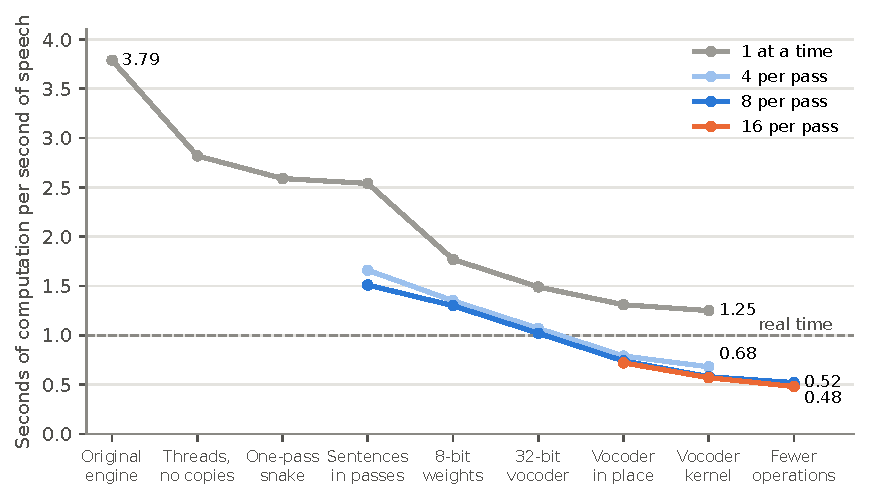
\includegraphics[width=0.9\textwidth,height=\textheight]{fig3_speed.pdf}
\caption{Speed of the engine as each group of revisions was added, one
sentence at a time and in passes of four, eight and 16. The dashed line
marks real time.}\label{fig:speed}
}
\end{figure}

The gains came in three phases. Removing waste took the engine from 3.79
to 2.82 seconds per second of speech one sentence at a time without
changing a sample, and the one-pass activation with a faster sine took
it to 2.59. Passes and 8-bit weights then addressed the memory limit,
and the vocoder revisions addressed the arithmetic limit, which had
become about half the time once passes were in use. Finally, replacing
many small operations with a few large ones took passes from 0.57 to
0.48. Beyond eight sentences, passes gained little until the operations
were merged, because the number of small operations grew with every
sentence added.

\hypertarget{combinations-of-the-newest-revisions}{%
\subsection{Combinations of the newest
revisions}\label{combinations-of-the-newest-revisions}}

The newest revisions were tested in every combination, since revisions
that help alone can interfere when combined. Each of 16 combinations of
four settings was run twice on 16 sentences, with greedy decoding, in
shuffled and then reversed order. All 38 runs, including confirmation
runs, gave identical audio.

The fastest combination took a median of 35.2 seconds against 42.0 for
the earlier settings, a real-time factor of 0.48 against 0.57. In three
alternating confirmation pairs, the ratios were 0.850, 0.846 and 0.851,
so the gain was consistent. We estimated each setting's effect as a
ratio of times, averaged over the other settings. It was 0.917 for the
batched predictor attention, 0.963 for the ordered talker attention and
0.976 for 16 rather than 8 sentences per stream. Decoding finished
sentences beside the pass, which seemed likely to help, took 23\% more
time (ratio 1.229). Interactions between settings were small, between
0.984 and 1.037.

Figure 5 shows where the saving came from. The acoustic predictor's time
fell from 18.3 to 12.8 seconds and the talker's from 7.4 to 6.7, while
the vocoder's hardly changed. The vocoder, at 14.3 seconds, is now the
largest stage (41\%), followed by the predictor (36\%) and the talker
(19\%).

\begin{figure}[tbp]
\hypertarget{fig:stages}{%
\centering
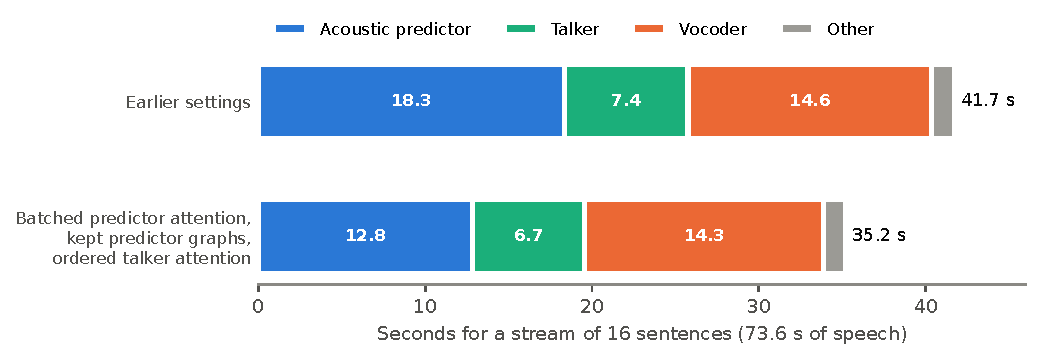
\includegraphics[width=0.85\textwidth,height=\textheight]{fig4_stages.pdf}
\caption{Where the time of a 16-sentence stream went, with the earlier
settings and with the batched predictor attention, kept predictor graphs
and ordered talker attention. Mean of the two confirmation runs of each
on the NUC.}\label{fig:stages}
}
\end{figure}

\hypertarget{full-lecture-recordings}{%
\subsection{Full lecture recordings}\label{full-lecture-recordings}}

The full lecture confirmed these gains (Table 3). The lecture had 51
slides and 578 sentences and was recorded several times as the revisions
were added. With the final settings and streams of 16, the NUC recorded
the 51.7-minute video in 30.2 minutes, 0.59 of its length, and the
finished video was ready in 31.4 minutes (0.61). With the settings
chosen by the combination test but all 15 predictor runs, the same
lecture had taken 32.6 minutes (0.63), and with the earlier settings
40.6 minutes (0.78). The predictor revisions therefore saved 20\%, close
to the 15\% of the matched short test. The final settings, which add 12
predictor runs, the take check and the kept talker graph, saved a
further 7\%. This is more than 12 runs alone were expected to give, and
run-to-run variation may account for part of it.

\begin{longtable}[]{@{}
  >{\raggedright\arraybackslash}p{(\columnwidth - 6\tabcolsep) * \real{0.5714}}
  >{\raggedleft\arraybackslash}p{(\columnwidth - 6\tabcolsep) * \real{0.1429}}
  >{\raggedleft\arraybackslash}p{(\columnwidth - 6\tabcolsep) * \real{0.1429}}
  >{\raggedleft\arraybackslash}p{(\columnwidth - 6\tabcolsep) * \real{0.1429}}@{}}
\caption{Recording times for the same 578-sentence lecture on the
NUC.}\tabularnewline
\toprule\noalign{}
\begin{minipage}[b]{\linewidth}\raggedright
Engine state
\end{minipage} & \begin{minipage}[b]{\linewidth}\raggedleft
Video (min)
\end{minipage} & \begin{minipage}[b]{\linewidth}\raggedleft
Recording (min)
\end{minipage} & \begin{minipage}[b]{\linewidth}\raggedleft
Recording / video
\end{minipage} \\
\midrule\noalign{}
\endfirsthead
\toprule\noalign{}
\begin{minipage}[b]{\linewidth}\raggedright
Engine state
\end{minipage} & \begin{minipage}[b]{\linewidth}\raggedleft
Video (min)
\end{minipage} & \begin{minipage}[b]{\linewidth}\raggedleft
Recording (min)
\end{minipage} & \begin{minipage}[b]{\linewidth}\raggedleft
Recording / video
\end{minipage} \\
\midrule\noalign{}
\endhead
\bottomrule\noalign{}
\endlastfoot
8-bit weights, 32-bit vocoder, 4 per pass & 51.6 & 56.2 & 1.09 \\
vocoder read in place, fixed passes of 8 & 51.5 & 44.4 & 0.86 \\
vocoder kernel, streams of 8, first run & 51.8 & 37.2 & 0.72 \\
vocoder kernel, streams of 8, second run & 51.6 & 35.3 & 0.68 \\
same revisions, streams of 16 & 51.8 & 40.6 & 0.78 \\
fewer and larger operations, streams of 16 & 51.8 & 32.6 & 0.63 \\
final: 12 predictor runs, take check, kept talker graph, streams of 16 &
51.7 & 30.2 & 0.59 \\
\end{longtable}

Runs with the same settings varied more than we expected. The two runs
with streams of eight differed by 5\%. The run with streams of 16 and
the same arithmetic was slower than both, although 16 sentences per
stream were faster than eight in short tests. A matched test also found
the engine builds used in these runs equal in speed. The computer's
temperature, its power management and other programs were not
controlled, so a single lecture can differ from another by up to about
15\% for reasons unrelated to the engine. Short matched tests with
alternating order are therefore the better guide to the effect of a
revision, and lectures the guide to what a user will see. In every run,
the slide videos were encoded during the recording, so rendering ended
within 1.2 minutes of the last take; in the final run, the last slide
video was ready 10.8 seconds after the last take.

\hypertarget{comparison-with-gemini-tts}{%
\subsection{Comparison with Gemini
TTS}\label{comparison-with-gemini-tts}}

How fast Gemini TTS recorded the lecture depended on how the application
called it (Table 4). With one sentence per request and one request in
flight, as the local engine receives its work, recording took 37.0
minutes for a 52.4-minute video (0.71). With RealMe Studio's default,
several sentences per request and two requests in flight, recording took
12.9 minutes for a 45.3-minute video (0.29). Nothing about the service
changed between the two runs. The speech cost US\$0.83 and US\$0.72,
against nothing with the local engine.

\begin{longtable}[]{@{}
  >{\raggedright\arraybackslash}p{(\columnwidth - 6\tabcolsep) * \real{0.1892}}
  >{\raggedright\arraybackslash}p{(\columnwidth - 6\tabcolsep) * \real{0.2703}}
  >{\raggedright\arraybackslash}p{(\columnwidth - 6\tabcolsep) * \real{0.2703}}
  >{\raggedright\arraybackslash}p{(\columnwidth - 6\tabcolsep) * \real{0.2703}}@{}}
\caption{The local engine and Gemini TTS, used in two ways, narrating
the same lecture script.}\tabularnewline
\toprule\noalign{}
\begin{minipage}[b]{\linewidth}\raggedright
\end{minipage} & \begin{minipage}[b]{\linewidth}\raggedright
Local engine
\end{minipage} & \begin{minipage}[b]{\linewidth}\raggedright
Gemini TTS, one sentence per request
\end{minipage} & \begin{minipage}[b]{\linewidth}\raggedright
Gemini TTS, grouped (default)
\end{minipage} \\
\midrule\noalign{}
\endfirsthead
\toprule\noalign{}
\begin{minipage}[b]{\linewidth}\raggedright
\end{minipage} & \begin{minipage}[b]{\linewidth}\raggedright
Local engine
\end{minipage} & \begin{minipage}[b]{\linewidth}\raggedright
Gemini TTS, one sentence per request
\end{minipage} & \begin{minipage}[b]{\linewidth}\raggedright
Gemini TTS, grouped (default)
\end{minipage} \\
\midrule\noalign{}
\endhead
\bottomrule\noalign{}
\endlastfoot
Where speech is computed & the user's computer, CPU only & Google's
servers & Google's servers \\
Units of work & 578 sentences, streams of 16 & 608 takes, 1 in flight
(12 re-recorded) & 84 requests of up to 738 characters, 2 in flight \\
Video from the same script & 51.7 min & 52.4 min & 45.3 min \\
Recording (share of video) & 30.2 min (0.59) & 37.0 min (0.71) & 12.9
min (0.29) \\
Finished video (share of video) & 31.4 min (0.61) & 46.7 min (0.89) &
22.3 min (0.49) \\
Cost of speech for this lecture & none & US\$0.83 & US\$0.72 \\
Privacy & nothing leaves the computer & voice and text sent to the
provider & as for one sentence \\
Reproducibility & the same engine and settings give the same samples
with sampling off & the model is controlled by the provider & as for one
sentence \\
\end{longtable}

Grouping made both voices faster, but for different reasons (Figure 6).
For Gemini, the time per request was about 2.3 seconds plus 0.30 seconds
per second of audio, so grouping spread a fixed cost per request over
more speech. For the local engine, grouping shared the memory traffic of
each step. Both leveled off after six to eight sentences, and in both
the useful size of a group was set by something other than speed.
Requests to Gemini of seven or more sentences came back about 9\%
hurried, which is why the application limits a request to 738
characters.

\begin{figure}[tbp]
\hypertarget{fig:grouping}{%
\centering
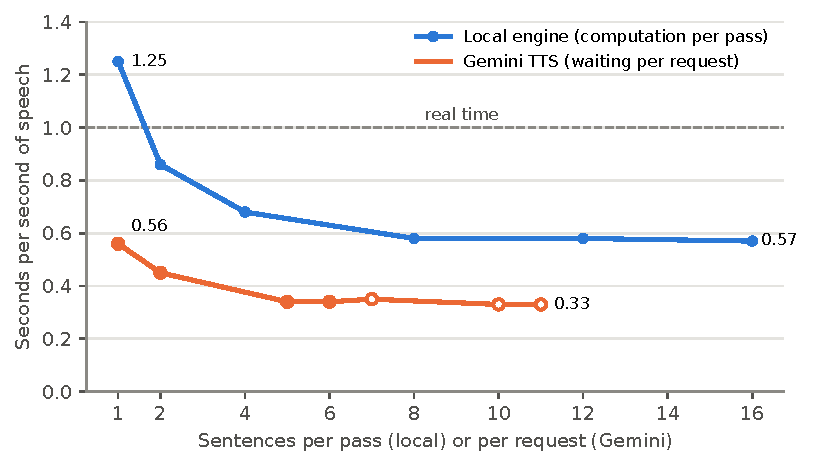
\includegraphics[width=0.85\textwidth,height=\textheight]{fig5_grouping.pdf}
\caption{Time per second of speech by the number of sentences grouped,
for Gemini TTS (waiting time per request, probe of 6 October 2026) and
the local engine before the revisions of Section 4.4 (computation time
per pass). Open circles: Gemini requests that came back
hurried.}\label{fig:grouping}
}
\end{figure}

On equal terms, the local engine was now faster than the hosted one.
With one sentence per request, Gemini needed 0.71 of the video's length,
against 0.59 for the local engine on a 15-watt processor, although each
figure rests on one run. Gemini's advantage in its default use, 0.29,
came from the application's grouping and concurrency rather than from
the speed of the hosted voice engine itself.

\hypertarget{voice-quality}{%
\subsection{Voice quality}\label{voice-quality}}

The revisions did not change the voice audibly. The exact revisions
reproduced the original waveform samples, and the others moved the
output 50 to 70 dB below the speech. In side-by-side listening, 8-bit
weights were not told apart from 16-bit weights, and 12 predictor runs
were not told apart from 15. The instructor listened to the lecture
recordings and judged the voice acceptable. No formal listening test was
carried out.

Variation from take to take was larger than any effect of the exact
revisions. With sampling on, as in normal use, each take of a sentence
differs in timing and emphasis; one passage lasted between 9.6 and 12.0
seconds across takes. Pronunciation depended more on text preparation
than on the engine. In the final run, the automatic audio check found no
mispronounced term but could not confirm four specialist terms, as with
the hosted voice. Two respellings had been corrected earlier after a
phonemizer check.

\hypertarget{discussion}{%
\section{Discussion}\label{discussion}}

This study showed that a capable open-weight model can do practical work
on a low-cost computer without a paid service. An instructor's cloned
voice narrated a 51.7-minute lecture in 30.2 minutes of recording on a
15-watt laptop processor, at no cost per use and without the voice
leaving the computer. The original engine would have needed more than
three hours. The difference came from software design and engineering,
not from better hardware: the model, the computer and, for most
revisions, the waveform samples stayed the same. To our knowledge, this
is the first detailed account of what limits a speech model of this kind
on a CPU. It also shows how each limit can be addressed while the output
stays verifiably unchanged.

\hypertarget{most-of-the-speed-was-in-the-software}{%
\subsection{Most of the speed was in the
software}\label{most-of-the-speed-was-in-the-software}}

Most of the gain of about 8 times came from how the software used the
hardware. Only the innermost tiles of two kernels, the 8-bit pass kernel
and the vocoder tile, are processor-specific, and without them the
engine kept about 80\% of its speed. The rest came from arranging the
work. Sentences shared each read of the weights, places were refilled as
sentences ended, conversions and copies were removed, and thousands of
small operations became a few large ones. Each of these is a design
decision rather than a property of the processor.

The application showed the same pattern at a higher level. The same
hosted service recorded the same lecture in 12.9 instead of 37.0 minutes
when the application grouped sentences and kept two requests in flight.
The local engine's largest single gain, passes, is the same kind of
decision as Gemini's grouped requests. In both cases, the simplest
working program, one sentence at a time and one task after another, was
correct but several times slower than it needed to be.

The engine was already six and a half times as fast when the newest
round of work began. Even so, looking at where the time went rather than
at the arithmetic cut the lecture's recording by another quarter, from
40.6 to 30.2 minutes. The acoustic predictor spent its time organizing
about 20,000 small operations per step, and a change that gave identical
numbers removed five sixths of them. This suggests that the room for
engineering is far from exhausted, in this engine and in others built
the same way.

This matters because programs are increasingly written with AI coding
assistants, a practice often called vibe coding, in which the developer
describes what is wanted and accepts program code that works. Such code
tends to take the simplest path to the right output. It passes every
functional test and may still waste most of the time it runs. The
original engine's thread count, stored but never applied, is the kind of
defect that only a timing measurement reveals. The same assistants did
the tuning reported here well when they were asked and directed by
measurements. The point is that someone has to ask.

\hypertarget{a-gpu-is-not-required-for-batch-work}{%
\subsection{A GPU is not required for batch
work}\label{a-gpu-is-not-required-for-batch-work}}

For producing a narrated lecture, the local engine on a laptop processor
was now faster than the hosted service used one sentence at a time (0.59
vs 0.71 of the video's length, one run each). The Qwen team's figure for
a GPU, a real-time factor of 0.29 for one streaming request, is also
within a factor of two of the 0.48 reached here. The two measures
differ, since theirs is the delay of a streaming request and ours the
throughput of a batch. Still, they place a laptop processor and a GPU
server in the same practical range for this task.

Two features of the task make this possible. The model is small and runs
at a low frame rate, so its weights fit easily in memory. More
importantly, lecture narration is batch work: all sentences are known in
advance, and none is needed at once. Processing sentences together turns
the memory limit of one sentence into a shared cost, which a CPU can
exploit as well as a GPU can. One sentence alone still needed 1.25
seconds per second of speech. Where a voice must answer at once, as in a
conversational agent, a GPU or a hosted service keeps a clear advantage.

The same reasoning applies to the choice of model. For English
narration, the 0.6-billion-parameter model was sufficient, and the
larger model would roughly triple the transformers' work. Choosing the
smallest model that meets the task, judged by the task's own criteria,
is also a design decision, and often the cheapest one.

\hypertarget{every-stage-can-be-tuned-with-checks}{%
\subsection{Every stage can be tuned, with
checks}\label{every-stage-can-be-tuned-with-checks}}

The model is a chain of stages, and each can be adjusted once it is
measured separately. Twelve predictor runs instead of 15 saved a fifth
of the predictor's steps with no audible change. The gain on a lecture
is modest, a few percent by the predictor's share, but it shows that
even the model's own structure is open to tuning, provided a check
guards the result. The take check makes such tuning safe: a take that
runs on or falls silent is caught in about a millisecond and recorded
again with the full model.

Checks mattered as much as the revisions. Requiring identical samples
made each exact revision testable in seconds and reversible at run time,
and it caught errors that listening would have missed. Exactness checks
are necessary but not sufficient, however. An independent review found
that the GPU vocoder option, as first written, ran every operation on
the CPU, because the weights stayed in the computer's memory. The
exactness test passed because the CPU fallback was exact, so only a
check of where the operations ran revealed the error. A change that
cannot be verified cannot be trusted, however fast it looks.

Consolidation was part of the same discipline. Experiments had produced
three builds of the engine and several model formats that gave the same
speed. Keeping one engine and removing the code that no longer earned
its place made the result easier to build, test and explain, without
changing an audio token.

\hypertarget{not-every-idea-pays}{%
\subsection{Not every idea pays}\label{not-every-idea-pays}}

Many plausible ideas did not pay, and only measurement separated them
from those that did. Decoding finished sentences beside the pass seemed
to overlap two stages for free, but it took 23\% more time, because both
stages competed for the same six cores. Four-bit weights were faster for
one sentence but slower in passes, where arithmetic rather than memory
sets the pace. Of 19 weight-layout and lookup options, none repeated a
gain of 3\% in two confirmations, possibly because an earlier kernel had
already taken the gain they aimed at. The twentieth, the ordered talker
attention, failed its first confirmation alone but helped consistently
in combination. More threads than physical cores made the engine slower.

These negative results are part of the finding. Whether an optimization
helps depends on which resource limits the work at that moment, and that
changes as other revisions are made. A gain measured alone can vanish in
combination, and a gain measured once can fail to repeat. Testing
settings in every combination, with repeated and alternating runs, was
what made the final choice reliable.

\hypertarget{implications-for-local-language-models-and-for-model-design}{%
\subsection{Implications for local language models and for model
design}\label{implications-for-local-language-models-and-for-model-design}}

The same reasoning extends to language models, which teaching and
research use far more widely than speech synthesis. A language model
also generates tokens one at a time, and each step reads the whole model
and does little arithmetic per byte. Processing several pieces of work
together, using 8-bit weights, removing redundant conversions and
merging small operations should therefore help in the same way. Much
academic work is also batch work: drafting slide notes, summarizing a
set of articles or classifying free-text answers can run overnight, like
a lecture recording. The differences make the task harder. Useful
language models are 10 to 100 times larger, and a small numerical change
can alter a text token and everything after it. Local language models
therefore need the same verification as here: outputs checked against a
reference with sampling fixed, and every lossy change measured on the
task itself.

The profile also suggests changes to the models themselves. The acoustic
predictor's 15 sequential runs carried most of the generation work.
Designs that predict several acoustic tokens in one step would shorten
this chain, and our listening test suggests that the finest codebooks
contribute little. Draft heads trained to guess several tokens at once,
which recent work suggests can be added to multi-token training at
almost no cost, are another route {[}6{]}. Quantization-aware training
would let implementations use smaller formats with confidence. Batched
synthesis that gives exactly the output of a single sentence would let
servers batch freely. Model developers mostly report speed on server
GPUs at full precision. Reporting speed and accuracy on modest hardware
and in reduced precision as well would show users which models suit
them.

\hypertarget{newer-hardware-and-future-work}{%
\subsection{Newer hardware and future
work}\label{newer-hardware-and-future-work}}

The engine is ready for, but not yet measured on, newer processors. On a
2025 Intel Core Ultra laptop, the build will compile the VNNI kernels
and share work between fast and slow cores. There, the 8-bit vocoder,
about 1.6 times as fast with VNNI in a synthetic test, may become a
default if listening confirms it. On an Apple M4 or M5 laptop, the ARM
kernels were checked only on an emulator, and a build path for macOS
remains to be written. With a GPU, the vocoder can run there while the
transformers stay on the CPU. A streaming vocoder, which would decode
each frame as it is generated, gained at most about 5\% on the CPU and
is better re-evaluated where a GPU makes the overlap free. Merging each
layer's products into one operation per pass is the most promising
remaining CPU change, since the transformers still run at under 10\% of
the processor's 8-bit peak.

\hypertarget{strengths-and-limitations}{%
\subsection{Strengths and limitations}\label{strengths-and-limitations}}

The main strength of this study is that every revision was measured on
real speech and checked against the original engine. The result was also
tested on a complete lecture rather than on isolated sentences. The
program code is public, with a switch for each revision, so the
measurements can be repeated on other computers.

The study also has limitations. First, all timings come from one
computer with a 15-watt, 6-core processor; other processors and power
budgets may give different gains, and ARM and GPU builds were verified
but not timed. Second, voice quality was judged by informal listening
and by PESQ rather than by a blinded test with several listeners, so
small differences may have gone unnoticed. Third, each full-lecture
configuration was recorded once or twice, and lectures with similar
settings differed by up to about 15\%. The lecture times therefore show
what a user will see rather than the precise effect of each revision.
Fourth, the comparison with Gemini TTS rests on one run of each
configuration, and the hosted service's speed depends on its load.
Fifth, the final settings were recorded on one lecture only, and that
run did not report how many takes the take check sent back for
recording.

\hypertarget{conclusion}{%
\section{Conclusion}\label{conclusion}}

An open-weight voice model, adapted to an ordinary laptop processor,
recorded a 51.7-minute narrated lecture in 0.59 of its length, at no
cost per use and with no data leaving the computer. The engine became
about 8 times as fast without new hardware and, for most revisions,
without changing a waveform sample, because most of the gain came from
software design and engineering. Whether a model runs locally or
remotely, measuring where the time goes, sharing the limiting resource
and verifying every change against a reference can change its speed
several times over. Much of that work remains to be done.

\hypertarget{declaration-on-the-use-of-ai-tools}{%
\section*{Declaration on the use of AI
tools}\label{declaration-on-the-use-of-ai-tools}}
\addcontentsline{toc}{section}{Declaration on the use of AI tools}

Program investigation, coding, measurement and testing in this study
were assisted by Claude Code (Anthropic), with some experiments carried
out by Codex (OpenAI). The project's research logs and reports, kept
throughout the work, were the foundation for the first draft of this
paper, which was written with Claude. The author directed the work,
listened to the recordings, edited the draft, checked its figures
against the logs and measurement files, and takes responsibility for its
content.

\hypertarget{references}{%
\section*{References}\label{references}}
\addcontentsline{toc}{section}{References}

\begin{enumerate}
\def\labelenumi{\arabic{enumi}.}
\tightlist
\item
  Qwen Team. Qwen3-TTS technical report. arXiv:2601.15621, January 2026.
  \url{https://arxiv.org/abs/2601.15621}
\item
  predict-woo. qwen3-tts.cpp: Qwen3-TTS in C++ on GGML (MIT license),
  commit b3ba14077cf1.
  \url{https://github.com/predict-woo/qwen3-tts.cpp}
\item
  The ggml authors. GGML tensor library (MIT license), commit
  3af5f5760e19. \url{https://github.com/ggml-org/ggml}
\item
  Google. Voice replication, Gemini API documentation.
  \url{https://ai.google.dev/gemini-api/docs/voice-replication}
\item
  Rix AW, Beerends JG, Hollier MP, Hekstra AP. Perceptual evaluation of
  speech quality (PESQ): a new method for speech quality assessment of
  telephone networks and codecs. Proceedings of ICASSP 2001; 2:749-752.
\item
  Teoh J. Multi-token prediction done right. arXiv:2610.38331, October
  2026. \url{https://arxiv.org/abs/2610.38331}
\item
  Yu X. realme-qwen3-tts.cpp: a revised qwen3-tts.cpp for ordinary CPUs.
  \url{https://github.com/xinhuayu/realme-qwen3-tts}
\end{enumerate}

Code availability. The revised engine, with its change list, run-time
switches, tests and a voice server that follows OpenAI's speech
interface, is available at
\url{https://github.com/xinhuayu/realme-qwen3-tts}. Each revision is
listed in its CHANGES.md with the files it touches, its effect on the
samples and the switch that turns it off.

\end{document}
